\documentclass{scrartcl}

\usepackage[utf8]{inputenc}

\usepackage{fixltx2e}

% Step environment
% <https://tex.stackexchange.com/a/12943/13262>
\usepackage{amsthm}
\newtheorem*{remark}{Remark}
%
\newtheoremstyle{named}{}{}{\itshape}{}{\bfseries}{.}{.5em}{\thmnote{#1 }#3}
\theoremstyle{named}
\newtheorem*{step}{Step}

\usepackage{microtype}
\usepackage{amsmath}
\usepackage{mathtools}
\usepackage{booktabs}
\usepackage{tabularx}

\usepackage{pgfplots}
\pgfplotsset{compat=newest}

\usepackage{siunitx}

\newcommand\mytitle{Remarks on the conversion from OSA-UCS to CIEXYZ}
\newcommand\myauthor{Nico Schlömer}

\usepackage[
  pdfencoding=unicode,
  ]{hyperref}
\hypersetup{
  pdfauthor={\myauthor},
  pdftitle={\mytitle}
}

% <https://tex.stackexchange.com/a/43009/13262>
\DeclarePairedDelimiter\abs{\lvert}{\rvert}%

\usepackage[T1]{fontenc}
\usepackage{newtxtext}
\usepackage{newtxmath}

% degree symbol
\usepackage{gensymb}

% % <https://tex.stackexchange.com/a/413899/13262>
% \usepackage{etoolbox}
% \makeatletter
% \long\def\etb@listitem#1#2{%
%   \expandafter\ifblank\expandafter{\@gobble#2}
%     {}
%     {\expandafter\etb@listitem@i
%      \expandafter{\@secondoftwo#2}{#1}}}
% \long\def\etb@listitem@i#1#2{#2{#1}}
% \makeatother

% Okay. Don't use biblatex/biber for now. There are breaking changes in every
% revision, and we'd have to stick to the exact version that arxiv.org has,
% otherwise it's error messages like
% ```
% Package biblatex Warning: File 'main.bbl' is wrong format version
% - expected 2.8.
% ```
% \usepackage[sorting=none]{biblatex}
% \bibliography{bib}

\usepackage{amsmath}
\DeclareMathOperator{\sign}{sign}

\usepackage{bm}
\newcommand\rgb{\bm{R}}

\title{\mytitle\footnote{The LaTeX sources of this article are on \url{https://github.com/nschloe/colorio}}}
\author{\myauthor}

\begin{document}

\maketitle
\begin{abstract}
  This
\end{abstract}

In 1974, MacAdam published the definition of the OSA-UCS colorspace~\cite{macadam} that
tries to adhere particularly well to experimentally measured color distances, and
represents work that had been going on since the late 1940s.  One aspect of OSA-UCS is
the fact that the conversion from CIEXYZ coordinates into OSA-UCS Lgj coordinates is
straightforward, but the conversion the other way around is not. In fact, there is no
conversion method that works purely in elementary functions. Apparently, this had not
been a design goal of OSA-UCS.

In 2002, Kobayasi and Yosiki presented an OSA-UCS-to-CIEXYZ algorithm that leverages
Newton's method for solving nonlinear equation systems~\cite{kobayasi}. While the
algorithm is mostly in order, the article remains vague at important points and also
contains false assertions about the nature of the involved functions.

In 2013, Cao et al.\ compared Kobayasi's approach with some other, more complicated
methods based on artificial neural networks and found the latter to be
superior~\cite{cao}.

In the present note, the author aims to iron out the inaccuracies in Kobayasi's article
and shows that the Newton-based approach is indeed fully sufficient for the conversion
from OSA-UCS to CIEXYZ.

\section{The forward conversion}

The conversion from CIEXYZ coordinates to OSA-UCS Lgj coordinates is definied as
follows:

\begin{itemize}
  \item Compute $x$, $y$ coordinates via
    \[
      x = \frac{X}{X + Y + Z},\quad y = \frac{Y}{X + Y + Z}.
    \]
  \item Compute $K$ and $Y_0$ as
    \begin{equation}\label{eq:KY0}
      \begin{split}
        K &= 4.4934 x^2 + 4.3034 y^2 - 4.276 x y - 1.3744 x - 2.5643 y + 1.8103,\\
        Y_0 &= Y K
      \end{split}
    \end{equation}

  \item Compute $L'$ and $C$ as
    \begin{align}
        \label{eq:lc}
        L' &= 5.9 \left(\sqrt[3]{Y_0} - \frac{2}{3} + 0.042 \sqrt[3]{Y_0 - 30}\right)\\
        \nonumber
        C &= \frac{L'}{5.9 \left(\sqrt[3]{Y_0} - \frac{2}{3}\right)}.
    \end{align}
    Note that $L'$ is $L$ in the original article~\cite{macadam}.

  \item Compute RGB as
    \begin{equation}\label{eq:m}
      \begin{bmatrix}
        R\\
        G\\
        B
      \end{bmatrix}
      =
      M
      \begin{bmatrix}
        X\\
        Y\\
        Z
      \end{bmatrix}
      \quad\text{with}\quad
      M=\begin{bmatrix}
        +0.7990 & 0.4194 & -0.1648\\
        -0.4493 & 1.3265 & +0.0927\\
        -0.1149 & 0.3394 & +0.7170
      \end{bmatrix}.
    \end{equation}

  \item Compute $a$, $b$ as
    \begin{equation}\label{eq:ab}
      \begin{bmatrix}
        a\\
        b
      \end{bmatrix}
      =
      A
      \begin{bmatrix}
        \sqrt[3]{R}\\
        \sqrt[3]{G}\\
        \sqrt[3]{B}
      \end{bmatrix}
      \quad\text{with}\quad
      A = \begin{bmatrix}
        -13.7 & +17.7 & -4\\
        1.7 & +8 & -9.7
      \end{bmatrix}.
    \end{equation}

  \item Compute $L$, $g$, $j$ as
    \[
      L = \frac{L' - 14.3993}{\sqrt{2}},\quad g = Ca,\quad j = Cb.
    \]
\end{itemize}

\section{The backward conversion}

This section describes the conversion from the  $L$, $g$, $j$ to the $X$, $Y$, $Z$
coordinates and mostly sticks to Kobayasi~\cite{kobayasi} here.

Given $L$, we can first compute
\[
  L' = L \sqrt{2} + 14.3993.
\]
Equation~\eqref{eq:lc} gives the nonlinear relationship between $L'$ and $Y_0$ from
which we will retrieve $Y_0$. First set $t\coloneqq \sqrt[3]{Y_0}$ and solve $f(t)=0$
for $t$ using Newton's method with
\[
  \begin{split}
    f(t) &\coloneqq {\left(\frac{L'}{5.9} + \frac{2}{3} - t\right)}^3 - 0.042^3 (t^3 - 30)\\
    f'(t) &= -3 {\left(\frac{L'}{5.9} + \frac{2}{3} - t\right)}^2 - 0.042^3 3 t^2.
  \end{split}
\]
It is reasonable to assume that
\[
  t_0 = \frac{L'}{5.9} + \frac{2}{3}
\]
is a good initial guess for $t$ since the second term in $f(t)$ with $0.042^3$ is
probably small.
Indeed, in practical application it takes less than 10 Newton iterations to achieve
convergence up to a tolerance of $10^{-13}$.

From here, one can compute
\begin{equation}\label{eq:gather}
  Y_0 = t^3,\quad
  C = \frac{L'}{5.9 \left(t - \frac{2}{3}\right)},\quad
  a = \frac{g}{C},\quad
  b = \frac{j}{C}.
\end{equation}
With $a$ and $b$ at hand, it is now possible via equation~\eqref{eq:ab} to pin down
$(\sqrt[3]{R}, \sqrt[3]{G}, \sqrt[3]{B})$ to only one degree of freedom, $w$.

The exact value will be found by another Newton iteration. The function $\phi(w)$
of which a root needs to be found is defined as follows.
\begin{quotation}
  Append the matrix $A$~\eqref{eq:ab} with a row such that the new $3\times3$-matrix
  $\tilde{A}$ is nonsingular and solve
  \[
    \begin{bmatrix}
      a\\
      b\\
      w
    \end{bmatrix}
    =
    \tilde{A}
    \begin{bmatrix}
      \sqrt[3]{R}\\
      \sqrt[3]{G}\\
      \sqrt[3]{B}
    \end{bmatrix}
  \]
  (Kobayasi, for instance, appends $[1, 0, 0]$.) Then compute the tentative $X$, $Y$,
  $Z$ via~\eqref{eq:m} and further get the corresponding $Y_0$ from~\eqref{eq:KY0}. If
  the difference between the computed value and the one from~\eqref{eq:gather} is 0, the
  correct $w$ has been found.
\end{quotation}

Kobayasi states the function $\phi$ is ``monotone increasing, convex downward, and
smooth''. Unfortunately, none of this is true (see figure~\ref{fig:singularity}). In
fact, the function has a singularity at $w$ chosen such that the computed tentative
$X$, $Y$, $Z$ sum up to 0 while the individual values of $|X|, |Y|, |Z| > 0$. This
happens if the tentative $[R, G, B]$ is orthogonal on $[1,1,1] M^{-1}$.

Fortunately, it seems that the function is indeed convex right of the singularity such
that Newton's method will find the correct (largest) root if the initial guess $w_0$ is
chosen larger than the root. Since $w$ corresponds to $\sqrt[3]{R}$, it is
reasonable to chose $w_0$ to be the maximum possible value that $\sqrt[3]{R}$ can take,
namely that corresponding to $X=Y=100$, $Z=0$ (see~\ref{eq:m}), $w_0=\sqrt[3]{79.9 +
41.94}\approx 4.9575$.

\begin{figure}
  \centering
  % This file was created by tikzplotlib v0.8.5.
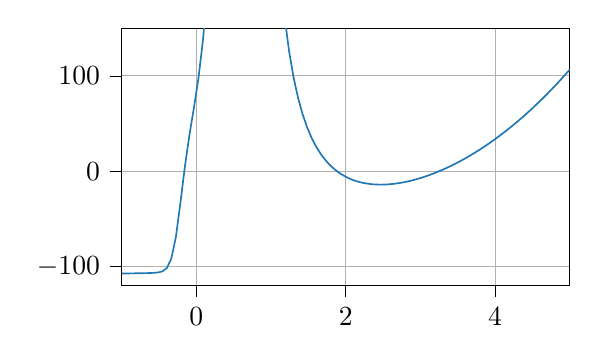
\begin{tikzpicture}

\definecolor{color0}{rgb}{0.12156862745098,0.466666666666667,0.705882352941177}

\begin{axis}[
width=0.6\textwidth,
height=0.4\textwidth,
tick align=outside,
tick pos=left,
x grid style={white!69.01960784313725!black},
xmajorgrids,
xmin=-1, xmax=5,
xtick style={color=black},
y grid style={white!69.01960784313725!black},
ymajorgrids,
ymin=-120, ymax=150,
ytick style={color=black}
]
\addplot [semithick, color0]
table {%
-1 -107.413027646396
-0.939393939393939 -107.309786831062
-0.878787878787879 -107.215237122039
-0.818181818181818 -107.127190104587
-0.757575757575758 -107.042359529441
-0.696969696969697 -106.954298360616
-0.636363636363636 -106.847025918721
-0.575757575757576 -106.673796503393
-0.515151515151515 -106.283050417142
-0.454545454545455 -105.164709350817
-0.393939393939394 -101.697626835742
-0.333333333333333 -91.7446608040379
-0.272727272727273 -69.1567235939574
-0.212121212121212 -33.4644220071798
-0.151515151515151 5.1529978523228
-0.0909090909090908 38.1524502469182
-0.0303030303030303 66.9186705474708
0.0303030303030303 97.8541264114677
0.0909090909090908 138.357047423149
0.151515151515152 197.483926762583
% 0.212121212121212 289.632097951798
% 0.272727272727273 442.766820835499
% 0.333333333333333 720.341273215897
% 0.393939393939394 1294.7437109525
% 0.454545454545455 2781.23788859758
% 0.515151515151515 8852.923932832
% 0.575757575757576 140918.648042227
% 0.636363636363636 39329.2370995238
% 0.696969696969697 6307.75066265103
% 0.757575757575758 2481.55333720743
% 0.818181818181818 1314.67993372474
% 0.878787878787879 807.312619103627
% 0.939393939393939 540.585092146669
% 1 382.62864181619
% 1.06060606060606 281.115967891114
% 1.12121212121212 211.877730132073
1.18181818181818 162.475784128249
1.24242424242424 125.967621812498
1.3030303030303 98.2246601475964
1.36363636363636 76.6635115820041
1.42424242424242 59.5986674360327
1.48484848484848 45.8913206375379
1.54545454545455 34.748884678301
1.60606060606061 25.6055084607501
1.66666666666667 18.048190278627
1.72727272727273 11.7696062648161
1.78787878787879 6.53714074322924
1.84848484848485 2.17204573916972
1.90909090909091 -1.46489446641638
1.96969696969697 -4.48341990771192
2.03030303030303 -6.97097581197619
2.09090909090909 -8.99792296863166
2.15151515151515 -10.6213738820869
2.21212121212121 -11.8880550669845
2.27272727272727 -12.836469002897
2.33333333333333 -13.4985456088261
2.39393939393939 -13.9009169725394
2.45454545454545 -14.0659108181188
2.51515151515152 -14.0123317432564
2.57575757575758 -13.7560807176327
2.63636363636364 -13.310650174996
2.6969696969697 -12.6875225826085
2.75757575757576 -11.8964935122321
2.81818181818182 -10.9459352060274
2.87878787878788 -9.84301290556648
2.93939393939394 -8.59386342878862
3 -7.20374338230765
3.06060606060606 -5.6771528032405
3.12121212121212 -4.01793880526886
3.18181818181818 -2.22938286355019
3.24242424242424 -0.314274643424397
3.3030303030303 1.72502529216217
3.36363636363636 3.88653200963904
3.42424242424242 6.16859043355976
3.48484848484849 8.56983602610926
3.54545454545455 11.0891608914696
3.60606060606061 13.7256844599801
3.66666666666667 16.4787280530134
3.72727272727273 19.3477927478875
3.78787878787879 22.3325400585856
3.84848484848485 25.4327750269647
3.90909090909091 28.6484313839621
3.96969696969697 31.9795584937718
4.03030303030303 35.4263098382213
4.09090909090909 38.9889328353565
4.15151515151515 42.6677598169073
4.21212121212121 46.4632000149567
4.27272727272727 50.375732429673
4.33333333333333 54.405899468091
4.39393939393939 58.5543012592435
4.45454545454546 62.8215905639128
4.51515151515152 67.2084682082878
4.57575757575758 71.7156789801974
4.63636363636364 76.3440079346035
4.6969696969697 81.0942770619015
4.75757575757576 85.9673422784606
4.81818181818182 90.9640907039071
4.87878787878788 96.0854381940253
4.93939393939394 101.332327101924
5 106.705724243391
};
\end{axis}

\end{tikzpicture}

  \caption{Graph of the function $\phi$ for $L$, $g$, $j$ computed from $X=12$, $Y=67$,
  $Z=20$. The singularity is as $w\approx 0.59652046418$. Note that the function as
  three roots.}\label{fig:singularity}
\end{figure}

\begin{figure}
  \centering
  \hfill
  % This file was created by tikzplotlib v0.8.5.
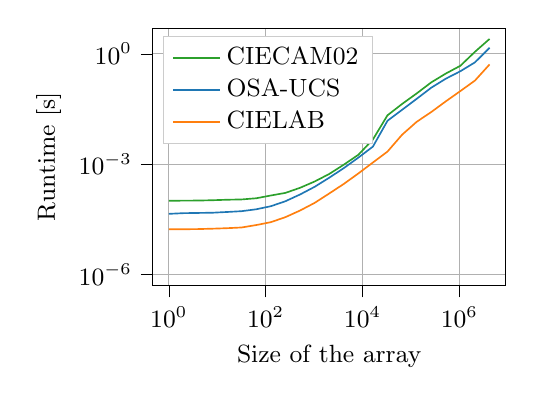
\begin{tikzpicture}
\small
\definecolor{color0}{rgb}{0.172549019607843,0.627450980392157,0.172549019607843}
\definecolor{color1}{rgb}{0.12156862745098,0.466666666666667,0.705882352941177}
\definecolor{color2}{rgb}{1,0.498039215686275,0.0549019607843137}
\definecolor{color3}{rgb}{0.83921568627451,0.152941176470588,0.156862745098039}

\begin{axis}[
width=0.5\textwidth,
height=0.4\textwidth,
legend cell align={left},
legend style={at={(0.03,0.97)}, anchor=north west, draw=white!80.0!black},
log basis x={10},
log basis y={10},
tick align=outside,
tick pos=left,
x grid style={white!69.01960784313725!black},
xmajorgrids,
xmin=0.466516495768404, xmax=8990687.44201965,
xmode=log,
xtick style={color=black},
y grid style={white!69.01960784313725!black},
xlabel={Size of the array},
ylabel={Runtime [s]},
ymajorgrids,
ymin=5.0e-07, ymax=5,
ymode=log,
ytick style={color=black}
]
\addplot [semithick, color0]
table {%
1 0.000100981
2 0.000102324
4 0.000102748
8 0.000104897
16 0.000108165
32 0.000110197
64 0.00011867
128 0.000141105
256 0.000166112
512 0.000228142
1024 0.000338372
2048 0.00054192
4096 0.00097015
8192 0.001803092
16384 0.004718868
32768 0.021407924
65536 0.043517433
131072 0.084103291
262144 0.168189022
524288 0.292563915
1048576 0.476608883
2097152 1.144089434
4194304 2.555706276
};
\addlegendentry{CIECAM02}
\addplot [semithick, color1]
table {%
1 4.4678e-05
2 4.6654e-05
4 4.7309e-05
8 4.797e-05
16 5.0236e-05
32 5.2868e-05
64 5.9526e-05
128 7.212e-05
256 9.8538e-05
512 0.000150111
1024 0.000242572
2048 0.000428417
4096 0.000782493
8192 0.001509464
16384 0.003013371
32768 0.015191504
65536 0.03020484
131072 0.059975308
262144 0.12048282
524288 0.212073153
1048576 0.338644042
2097152 0.589981183
4194304 1.468489001
};
\addlegendentry{OSA-UCS}
\addplot [semithick, color2]
table {%
1 1.6985e-05
2 1.7038e-05
4 1.7219e-05
8 1.765e-05
16 1.8212e-05
32 1.9048e-05
64 2.2169e-05
128 2.6533e-05
256 3.638e-05
512 5.4935e-05
1024 8.8606e-05
2048 0.00015956
4096 0.00029051
8192 0.000560139
16384 0.001113357
32768 0.002206901
65536 0.006332622
131072 0.014223582
262144 0.026245994
524288 0.051337911
1048576 0.097840739
2097152 0.188841351
4194304 0.516788318
};
\addlegendentry{CIELAB}
% \addplot [semithick, color3]
% table {%
% 1 5.9e-07
% 2 6.34e-07
% 4 7.51e-07
% 8 9.61e-07
% 16 1.363e-06
% 32 2.181e-06
% 64 3.891e-06
% 128 7.311e-06
% 256 1.4119e-05
% 512 2.7611e-05
% 1024 5.4443e-05
% 2048 0.000108013
% 4096 0.000215162
% 8192 0.00042941
% 16384 0.00085769
% 32768 0.001714179
% 65536 0.00352076
% 131072 0.007052502
% 262144 0.014110123
% 524288 0.027596741
% 1048576 0.054849061
% 2097152 0.109707066
% 4194304 0.228054266
% };
% \addlegendentry{cbrt}
\end{axis}

\end{tikzpicture}

  \hfill
  % This file was created by tikzplotlib v0.8.5.
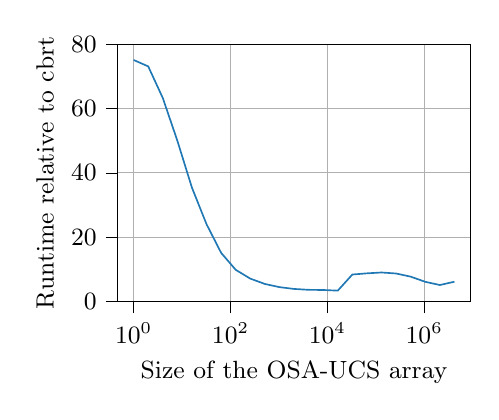
\begin{tikzpicture}
\small
\definecolor{color0}{rgb}{0.12156862745098,0.466666666666667,0.705882352941177}

\begin{axis}[
width=0.5\textwidth,
height=0.4\textwidth,
log basis x={10},
tick align=outside,
tick pos=left,
x grid style={white!69.01960784313725!black},
xmajorgrids,
xmin=0.466516495768404, xmax=8990687.44201965,
xmode=log,
xtick style={color=black},
y grid style={white!69.01960784313725!black},
xlabel={Size of the OSA-UCS array},
ylabel={Runtime relative to cbrt},
ymajorgrids,
ymin=0, ymax=80,
ytick style={color=black}
]
\addplot [semithick, color0]
table {%
1 75.1006711409396
2 73.1083591331269
4 63.2708058124174
8 49.9710743801653
16 35.3772241992883
32 24.0321412403803
64 15.1508196721311
128 9.87406398910824
256 7.13691159586682
512 5.47668013220712
1024 4.49142500779545
2048 3.92909630369076
4096 3.65669148862134
8192 3.60371143996241
16384 3.40274732706172
32768 8.41146602915969
65536 8.77937404511574
131072 9.04530219257962
262144 8.72914301960624
524288 7.74882579040905
1048576 6.14407398357426
2097152 5.1461952341571
4194304 6.17645701530873
};
\end{axis}

\end{tikzpicture}

  \hfill
  \caption{Computation speed for arrays of $Lgj$ values measured with
  colorio~\cite{colorio}. Left: Comparison with CIELAB (faster) and CIECAM02 (slower).
  The conversion of several million $Lgj$ values takes about 1 second. Right:
  Computation speed relative to the evaluation of the cubic root. For large arrays, the
  conversion to $XYZ$ is about as costly as the evaluation of 6 cubic roots.}
\end{figure}

% \printbibliography{}
\bibliography{main}{}
\bibliographystyle{plain}

\end{document}
